% !TeX root = ../index.tex

\section{Connecting to the Virtual Machine}

\begin{enumerate}
  \item Login as \texttt{ubuntu}.

        \begin{minted}{text}
          $ ssh ubuntu@141.72.189.100
        \end{minted}

  \item Accept the server fingerprint by typing \texttt{yes}.
  \item Enter the password.
\end{enumerate}

\section{Common UNIX Commands}

\begin{description}
  \item[man] Displays pages of the system's reference manual.
  \item[pwd] Returns the \textbf{p}resent (i.~e. current) \textbf{w}orking \textbf{d}irectory.
  \item[ls] Displays the contents of a directory.
  \item[more] Filters text for viewing one \emph{screenful} at a time. Useful for terminals that do not allow scrolling.
  \item[mv] Moves files or directories. Can also be used to rename files or directories.
  \item[cp] Copies files or directories.
  \item[rm] Removes files or directories.
  \item[mkdir] Creates directories.
  \item[rmdir] Removes directories.
  \item[chmod] Changes the \emph{mode bits} of files and directories. Mode bits determine among other things a file or directory's access permissions.
  \item[ps] Displays the processes currently running.
  \item[kill] Terminates processes.
\end{description}

\begin{enumerate}
  \item What will happen if you type \texttt{man man} in UNIX/Linux?

        \texttt{man} will display the manual page of the \texttt{man} command---i.~e. its own manual page.

  \item How can you use the command \texttt{ls} to find out about the size of file \texttt{/etc/passwd}?

        \texttt{ls -lh /etc/passwd} shows the file size in human-readable units.

  \item What is the command to determine all processes that are running on the system?

        \texttt{ps -e} prints all processes currently running on the system.

  \item What does the command \texttt{more} do?

        See above.

  \item What happens if you have two files with names \texttt{file1} and \texttt{file2} and you type \texttt{mv file1 file2}? Which option of \texttt{mv} will issue a warning in this situation?

        The command moves (renames) \texttt{file1} to \texttt{file2} overwriting the latter's contents in the process.
        The \texttt{-i} option would prompt the user for confirmation if file contents would be overwritten by an operation.

  \item What is the command that you issue if you are in directory \texttt{/} and want to copy the file \texttt{/mydata} to directory \texttt{/labdata}?

        \texttt{cp -r mydata labdata}

  \item What does the command \texttt{kill -9 pid} do, where pid is the number of a process?

        It sends the \texttt{KILL} signal to the system causing it to immediately terminate the process identified by the PID.
        The process itself does not capture the signal and has no chance to react or gracefully shut down.

  \item What happens if you type the command \texttt{rm *} in a directory?

        The shell will recognize the \texttt{*} as a wildcard and replace it with every non-hidden file and directory in the working directory before invoking the \texttt{rm} command.

        \begin{minted}{text}
          # where
          $ ls -A
          dir1 file1 file2 .hidden
          # then
          $ rm *
          # is equivalent to
          $ rm dir1 file1 file2
        \end{minted}

  \item Familiarize yourself with one of the available text editors (e.~g. vi or nano). Create a simple file using the text editor.

        \begin{enumerate}
          \item Enter \texttt{vi hello-world.txt} to open a new vi buffer.
          \item Hit \texttt{i} to enter \emph{insert mode}.
          \item Enter \texttt{Hello World!}.
          \item Hit \texttt{ESC} to exit insert mode.
          \item Enter \texttt{:wq} to \textbf{w}rite the contents of the buffer to the file system and \textbf{q}uit the editor.
          \item \texttt{cat hello-world.txt} will print \texttt{Hello World!}.
        \end{enumerate}
\end{enumerate}

\section{Networking}

\subsection{Inspect the Network Interfaces}

The \texttt{ifconfig} command produces the following output on the first machine.

\begin{minted}{text}
  $ ifconfig
  docker0: flags=4099<UP,BROADCAST,MULTICAST>  mtu 1500
          inet 172.17.0.1  netmask 255.255.0.0  broadcast 172.17.255.255
          ether 02:42:3c:7e:7e:6d  txqueuelen 0  (Ethernet)
          RX packets 0  bytes 0 (0.0 B)
          RX errors 0  dropped 0  overruns 0  frame 0
          TX packets 0  bytes 0 (0.0 B)
          TX errors 0  dropped 0 overruns 0  carrier 0  collisions 0

  ens3: flags=4163<UP,BROADCAST,RUNNING,MULTICAST>  mtu 1450
          inet 192.168.0.168  netmask 255.255.255.0  broadcast 192.168.0.255
          inet6 fe80::f816:3eff:fe83:7e55  prefixlen 64  scopeid 0x20<link>
          ether fa:16:3e:83:7e:55  txqueuelen 1000  (Ethernet)
          RX packets 216662  bytes 939829626 (939.8 MB)
          RX errors 0  dropped 0  overruns 0  frame 0
          TX packets 142777  bytes 12252882 (12.2 MB)
          TX errors 0  dropped 0 overruns 0  carrier 0  collisions 0

  lo: flags=73<UP,LOOPBACK,RUNNING>  mtu 65536
          inet 127.0.0.1  netmask 255.0.0.0
          inet6 ::1  prefixlen 128  scopeid 0x10<host>
          loop  txqueuelen 1000  (Local Loopback)
          RX packets 27427  bytes 2895195 (2.8 MB)
          RX errors 0  dropped 0  overruns 0  frame 0
          TX packets 27427  bytes 2895195 (2.8 MB)
          TX errors 0  dropped 0 overruns 0  carrier 0  collisions 0
\end{minted}

The output shows three network interfaces: The local loopback interface \texttt{lo}, the Docker network interface \texttt{docker0} and the Ethernet interface \texttt{ens3}.
The machine is reachable via \texttt{ens3} but it shows \texttt{192.168.0.168} to be its IP address instead of \texttt{141.72.189.100} via which I am connected.
This is due to the machine being part of a subnet behind a virtual router in the OpenStack infrastructure.

\subsection{Pinging the Other Machine}

Pinging the other machine with:

\begin{minted}{text}
  # -c <count> ping the host only <count> times
  $  ping -c 8 141.72.189.239
  PING 141.72.189.239 (141.72.189.239) 56(84) bytes of data.
  64 bytes from 141.72.189.239: icmp_seq=1 ttl=59 time=5.01 ms
  64 bytes from 141.72.189.239: icmp_seq=2 ttl=59 time=4.34 ms
  64 bytes from 141.72.189.239: icmp_seq=3 ttl=59 time=4.15 ms
  64 bytes from 141.72.189.239: icmp_seq=4 ttl=59 time=2.64 ms
  64 bytes from 141.72.189.239: icmp_seq=5 ttl=59 time=3.30 ms
  64 bytes from 141.72.189.239: icmp_seq=6 ttl=59 time=3.07 ms
  64 bytes from 141.72.189.239: icmp_seq=7 ttl=59 time=2.68 ms
  64 bytes from 141.72.189.239: icmp_seq=8 ttl=59 time=3.57 ms

  --- 141.72.189.239 ping statistics ---
  8 packets transmitted, 8 received, 0% packet loss, time 7012ms
  rtt min/avg/max/mdev = 2.640/3.594/5.008/0.787 ms
\end{minted}

\subsection{Create a User on the First Machine}\label{sec:create-user}

\begin{enumerate}
  \item Create a new user \enquote{kevin} and assign it to the group \enquote{sudo} to give it super user privileges.

        \begin{minted}{text}
          # -m          create home directory
          # -s          specify login shell
          # -G <groups> assign groups
          $ sudo useradd -m -s /bin/text -G sudo kevin
        \end{minted}

  \item Set a password for the new user.

        \begin{minted}{text}
          $ sudo passwd kevin
        \end{minted}

  \item Switch to a new login session as \enquote{kevin}.

        \begin{minted}{text}
          # -H        move to user's home directory
          # -i        launch login shell
          # -u <user> switch to specified user
          $ sudo -Hiu kevin
        \end{minted}
\end{enumerate}

\subsection{Configure Key-based Access}

\begin{enumerate}
  \item Create the \enquote{ssh} directory in the user's home directory.

        \begin{minted}{text}
          $ pwd
          /home/kevin
          $ mkdir .ssh
        \end{minted}

  \item Generate a new SSH public/private key pair on the local machine.

        \begin{minted}{text}
          $ ssh-keygen -t rsa
          Generating public/private rsa key pair.
          Enter file in which to save the key (/home/kevin/.ssh/id_rsa): id_rsa-studentnode-3
          Enter passphrase (empty for no passphrase):
          Enter same passphrase again:
          Your identification has been saved in id_rsa-studentnode-3
          Your public key has been saved in id_rsa-studentnode-3.pub
          The key fingerprint is:
          SHA256:A2WCyEJyk6QZlsPppoKjAWARs0fgMzPF5fXi+GOLwps kevin@kevin-thinkpad
          The key's randomart image is:
          +---[RSA 3072]----+
          |=X@=.o..o        |
          |*@Ooo .+.        |
          |*O.. ... .       |
          |.o*   o..        |
          |=    . .S        |
          |*     .  .       |
          |oo.    +         |
          |.  o. o o        |
          |   Eo. .         |
          +----[SHA256]-----+
          $ ls -l .ssh
          -rw------- 1 kevin kevin 1679 Feb  3 13:14 id_rsa-studentnode-3
          -rw-r--r-- 1 kevin kevin  401 Feb  3 13:14 id_rsa-studentnode-3.pub
        \end{minted}

  \item Configure the local machine's SSH agent to use the new private key to authenticate when connecting to the virtual machine.

        \begin{minted}{text}
          $ cat >> ~/.ssh/config <<EOF
          Host studentnode-3
            IdentityFile ~/.ssh/id_rsa-studentnode-3
            Hostname     141.72.189.100
            User         kevin
       
          EOF
        \end{minted}

  \item Copy the public key from the local to the virtual machine.

        \begin{minted}{text}
          $ ssh-copy-id -i id_rsa-studentnode-3.pub kevin@studentnode-3
        \end{minted}

  \item Enable public key authentication and disable password authentication on the virtual machine.

        \begin{minted}{text}
          # Set 'PasswordAuthentication' to 'no'
          # Set 'PubkeyAuthentication' to 'yes'
          $ sudo vim /etc/ssh/sshd_config
        \end{minted}

  \item Quit the current SSH session and re-connect using public key authentication.

        \begin{minted}{text}
          # Quit the current session
          $ exit
          # Login anew
          $ ssh studentnode-3
        \end{minted}
\end{enumerate}

\subsection{Monitor Network Traffic}

\begin{enumerate}
  \item Create a user \enquote{joe} one the second virtual machine by repeating the steps in \ref{sec:create-user}.
  \item Install the Telnet daemon on the second machine.
        \begin{minted}{text}
          $ sudo apt install telnetd
        \end{minted}
  \item Start Wireshark on the first machine.

        \begin{itemize}
          \item If presented with an error message, reconfigure the Wireshark kernel module to allow non-root users.

                \begin{minted}{text}
                  $ sudo dpkg-reconfigure wireshark-common
                \end{minted}

          \item Assign your user to the \enquote{wireshark} group.

                \begin{minted}{text}
                  $ sudo usermod -aG wireshark kevin
                \end{minted}

          \item Launch Wireshark again.
        \end{itemize}

  \item Capture the traffic on \enquote{ens3} with Wireshark while interacting with the second machine via Telnet.
\end{enumerate}

\begin{figure}[H]
  \centering
  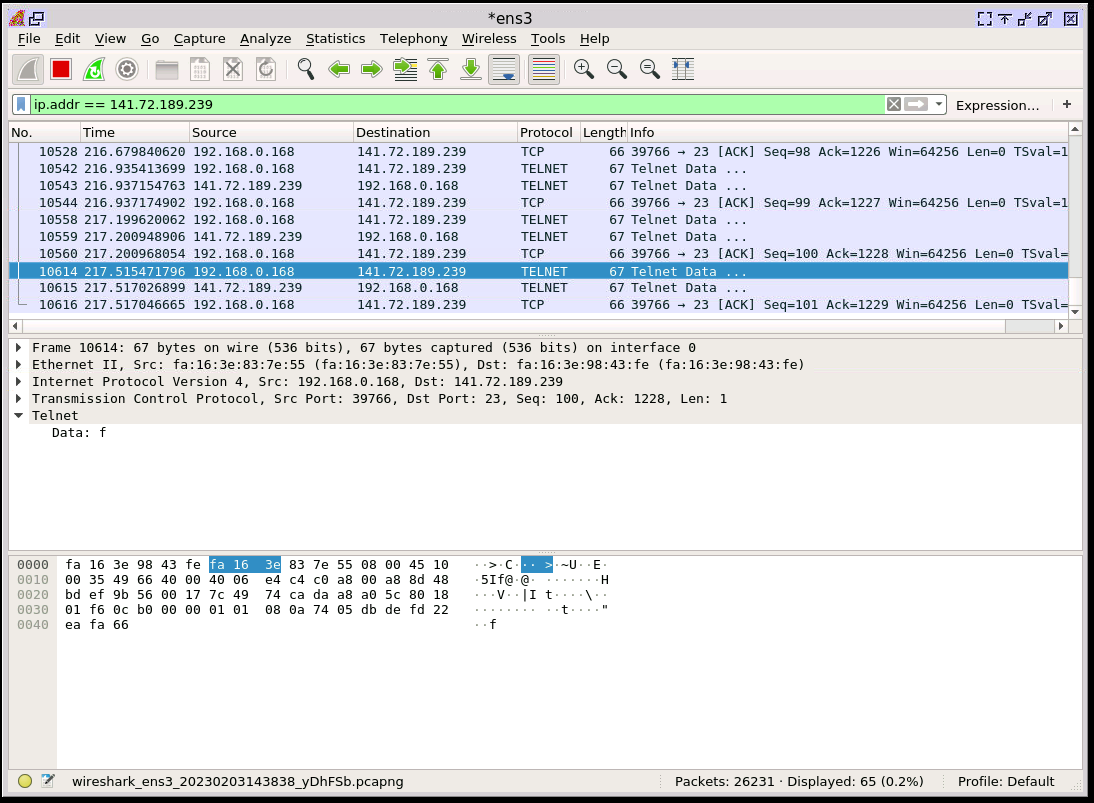
\includegraphics[width=0.9\textwidth]{wireshark-telnet.png}
  \caption{Screenshot of Wireshark capturing Telnet traffic}
  \label{fig:wireshark}
\end{figure}

Figure \ref{fig:wireshark} shows captured Telnet traffic.
The fact that individual characters in the traffic are clearly identifiable tells us that Telnet traffic is not encrypted.

